\documentclass[conference]{IEEEtran}
\usepackage[spanish]{babel}
\usepackage{cite}
\usepackage{amsmath,amssymb,amsfonts}
\usepackage{algorithmic}
\usepackage{graphicx}
\usepackage{textcomp}
\usepackage{xcolor}
\usepackage{booktabs}
\usepackage{tabularx}
\usepackage{hyperref}
\usepackage{multirow}

\def\BibTeX{{\rm B\kern-.05em{\sc i\kern-.025em b}\kern-.08em
    T\kern-.1667em\lower.7ex\hbox{E}\kern-.125emX}}

\title{GP-CPS: Un Framework de Gemelo Digital basado en\\ Procesos Gaussianos para Sistemas Ciber-Físicos Multi-Variable}

\author{\IEEEauthorblockN{J. Calataiut-Cl\raisebox{0.5mm}{\noindent\rule{3mm}{0.5pt}}i\raisebox{0.5mm}{\noindent\rule{3mm}{0.5pt}}}
\IEEEauthorblockA{Departamento de Matemáticas Avanzadas\\
Universidad Politécnica\\
Email: jcalataiut-cli@github.com}
}

\begin{document}

\maketitle

\begin{abstract}
Los gemelos digitales son réplicas virtuales de sistemas físicos que permiten simulación, predicción y detección de anomalías sin interrumpir operaciones reales. Los enfoques más avanzados utilizan modelos de difusión entrenados con series temporales multivariantes (MTS), requiriendo infraestructura GPU costosa y horas de entrenamiento. En este artículo proponemos \textbf{GP-CPS}, un framework que emplea Procesos Gaussianos (GP) como motor generativo para construir gemelos digitales de Sistemas Ciber-Físicos (CPS). Al reemplazar modelos de difusión por GP---que comparten una profunda conexión teórica con los Procesos Gaussianos de Redes Neuronales (NNGP)---nuestro enfoque logra rendimiento predictivo competitivo mientras reduce el tiempo de entrenamiento de horas a minutos en CPU. Evaluamos GP-CPS en un caso de estudio de Zona de Edificio Inteligente con cuatro variables interdependientes (temperatura, humedad, CO$_2$, ocupación). Nuestros resultados muestran $R^2 > 0.95$ para todas las variables, con errores absolutos medios de $0.23^\circ$C para temperatura y 20.7~ppm para CO$_2$, y demuestran detección efectiva de anomalías mediante la cuantificación de incertidumbre del GP. El framework se ejecuta completamente en hardware estándar sin necesidad de GPU, haciendo accesible la tecnología de gemelos digitales para prototipado rápido y entornos educativos.
\end{abstract}

\begin{IEEEkeywords}
Sistemas Ciber-Físicos, Gemelo Digital, Proceso Gaussiano, IA Generativa, Detección de Anomalías, NNGP
\end{IEEEkeywords}

\section{Introducción}
\label{sec:introduccion}

Los Sistemas Ciber-Físicos (CPS)---integración estrecha de computación, comunicación y procesos físicos---son fundamentales para la industria, el transporte y las infraestructuras modernas~\cite{lee2015, zhang2022}. El auge del Internet Industrial de las Cosas (IIoT) ha permitido flujos masivos de datos heterogéneos de sensores, capturando la complejidad del comportamiento del sistema a través de múltiples variables interdependientes que evolucionan en el tiempo.

Los enfoques tradicionales de simulación se basan en modelos analíticos explícitos de la dinámica del sistema. Sin embargo, los CPS modernos exhiben no-linealidades, comportamientos estocásticos y configuraciones evolutivas que hacen que los modelos artesanales sean cada vez más impracticables~\cite{yaacoub2020}. Las técnicas basadas en datos ofrecen una alternativa escalable: al aprender patrones directamente de los datos de sensores, pueden modelar distribuciones conjuntas de variables del sistema para simulación y predicción realistas~\cite{yuan2019}.

Trabajos recientes~\cite{turco2025} propusieron el uso de Modelos de Difusión (específicamente Rectified Flows) para construir gemelos digitales a partir de series temporales multivariantes, aplicado a un brazo robótico antropomórfico dentro de la plataforma de simulación Frost. Aunque efectivo, este enfoque requiere recursos computacionales significativos: entrenar modelos de difusión típicamente demanda horas de GPU, limitando la accesibilidad para prototipado rápido, contextos educativos y entornos con recursos limitados.

En este artículo, abordamos estas limitaciones introduciendo \textbf{GP-CPS}, un framework que reemplaza los modelos de difusión con Procesos Gaussianos (GP) como motor generativo para la construcción de gemelos digitales. Nuestras contribuciones son:

\begin{enumerate}
\item \textbf{Un framework generativo basado en GP para gemelos digitales CPS}, que requiere solo entrenamiento en CPU en minutos en lugar de horas de GPU.
\item \textbf{Un nuevo dominio de caso de estudio---Zona de Edificio Inteligente---reemplazando el brazo robótico}, demostrando aplicabilidad transversal.
\item \textbf{Detección de anomalías mediante cuantificación de incertidumbre del GP}, donde desviaciones más allá de $2\sigma$ señalan anomalías del sistema.
\item \textbf{Una conexión teórica con la teoría de Procesos Gaussianos de Redes Neuronales}, puenteando la aplicación de gemelos digitales con la literatura NNGP.
\end{enumerate}

\section{Antecedentes y Trabajo Relacionado}
\label{sec:antecedentes}

\subsection{Modelos Generativos para CPS}
Los modelos generativos han surgido como herramientas poderosas para la simulación de CPS. Los Autoencoders Variacionales (VAEs)~\cite{kingma2013} aprenden distribuciones latentes para generación diversa; los modelos Autorregresivos~\cite{oord2016} capturan dependencias temporales; las Redes Generativas Antagónicas (GANs)~\cite{goodfellow2014} enfrentan generador contra discriminador; y los Modelos de Difusión~\cite{ho2020} invierten iterativamente un proceso de corrupción. El framework Frost~\cite{turco2025,turco2025frost} ejemplifica el enfoque basado en difusión, usando Rectified Flows sobre Lingua Franca~\cite{lohstroh2021}.

\subsection{Procesos Gaussianos en Sistemas Dinámicos}
Los Procesos Gaussianos~\cite{rasmussen2006} proporcionan un marco Bayesiano no paramétrico para aprender funciones desconocidas a partir de datos. En sistemas dinámicos, los GP se han utilizado para identificación de sistemas~\cite{kocijan2004}, control~\cite{deisenroth2011} y modelado de series temporales. La ventaja clave es la cuantificación natural de incertidumbre a través de la varianza predictiva.

\subsection{Conexión con la Teoría NNGP}
La correspondencia NNGP (Neural Network Gaussian Process)~\cite{lee2018, jacot2018} establece que una red neuronal de ancho infinito converge a un Proceso Gaussiano. Este fundamento teórico conecta los enfoques basados en redes neuronales y los basados en GP. Nuestro trabajo aprovecha esta conexión utilizando GP directamente como modelo generativo, beneficiándose implícitamente de las garantías teóricas de NNGP.

\begin{figure}[t]
\centering
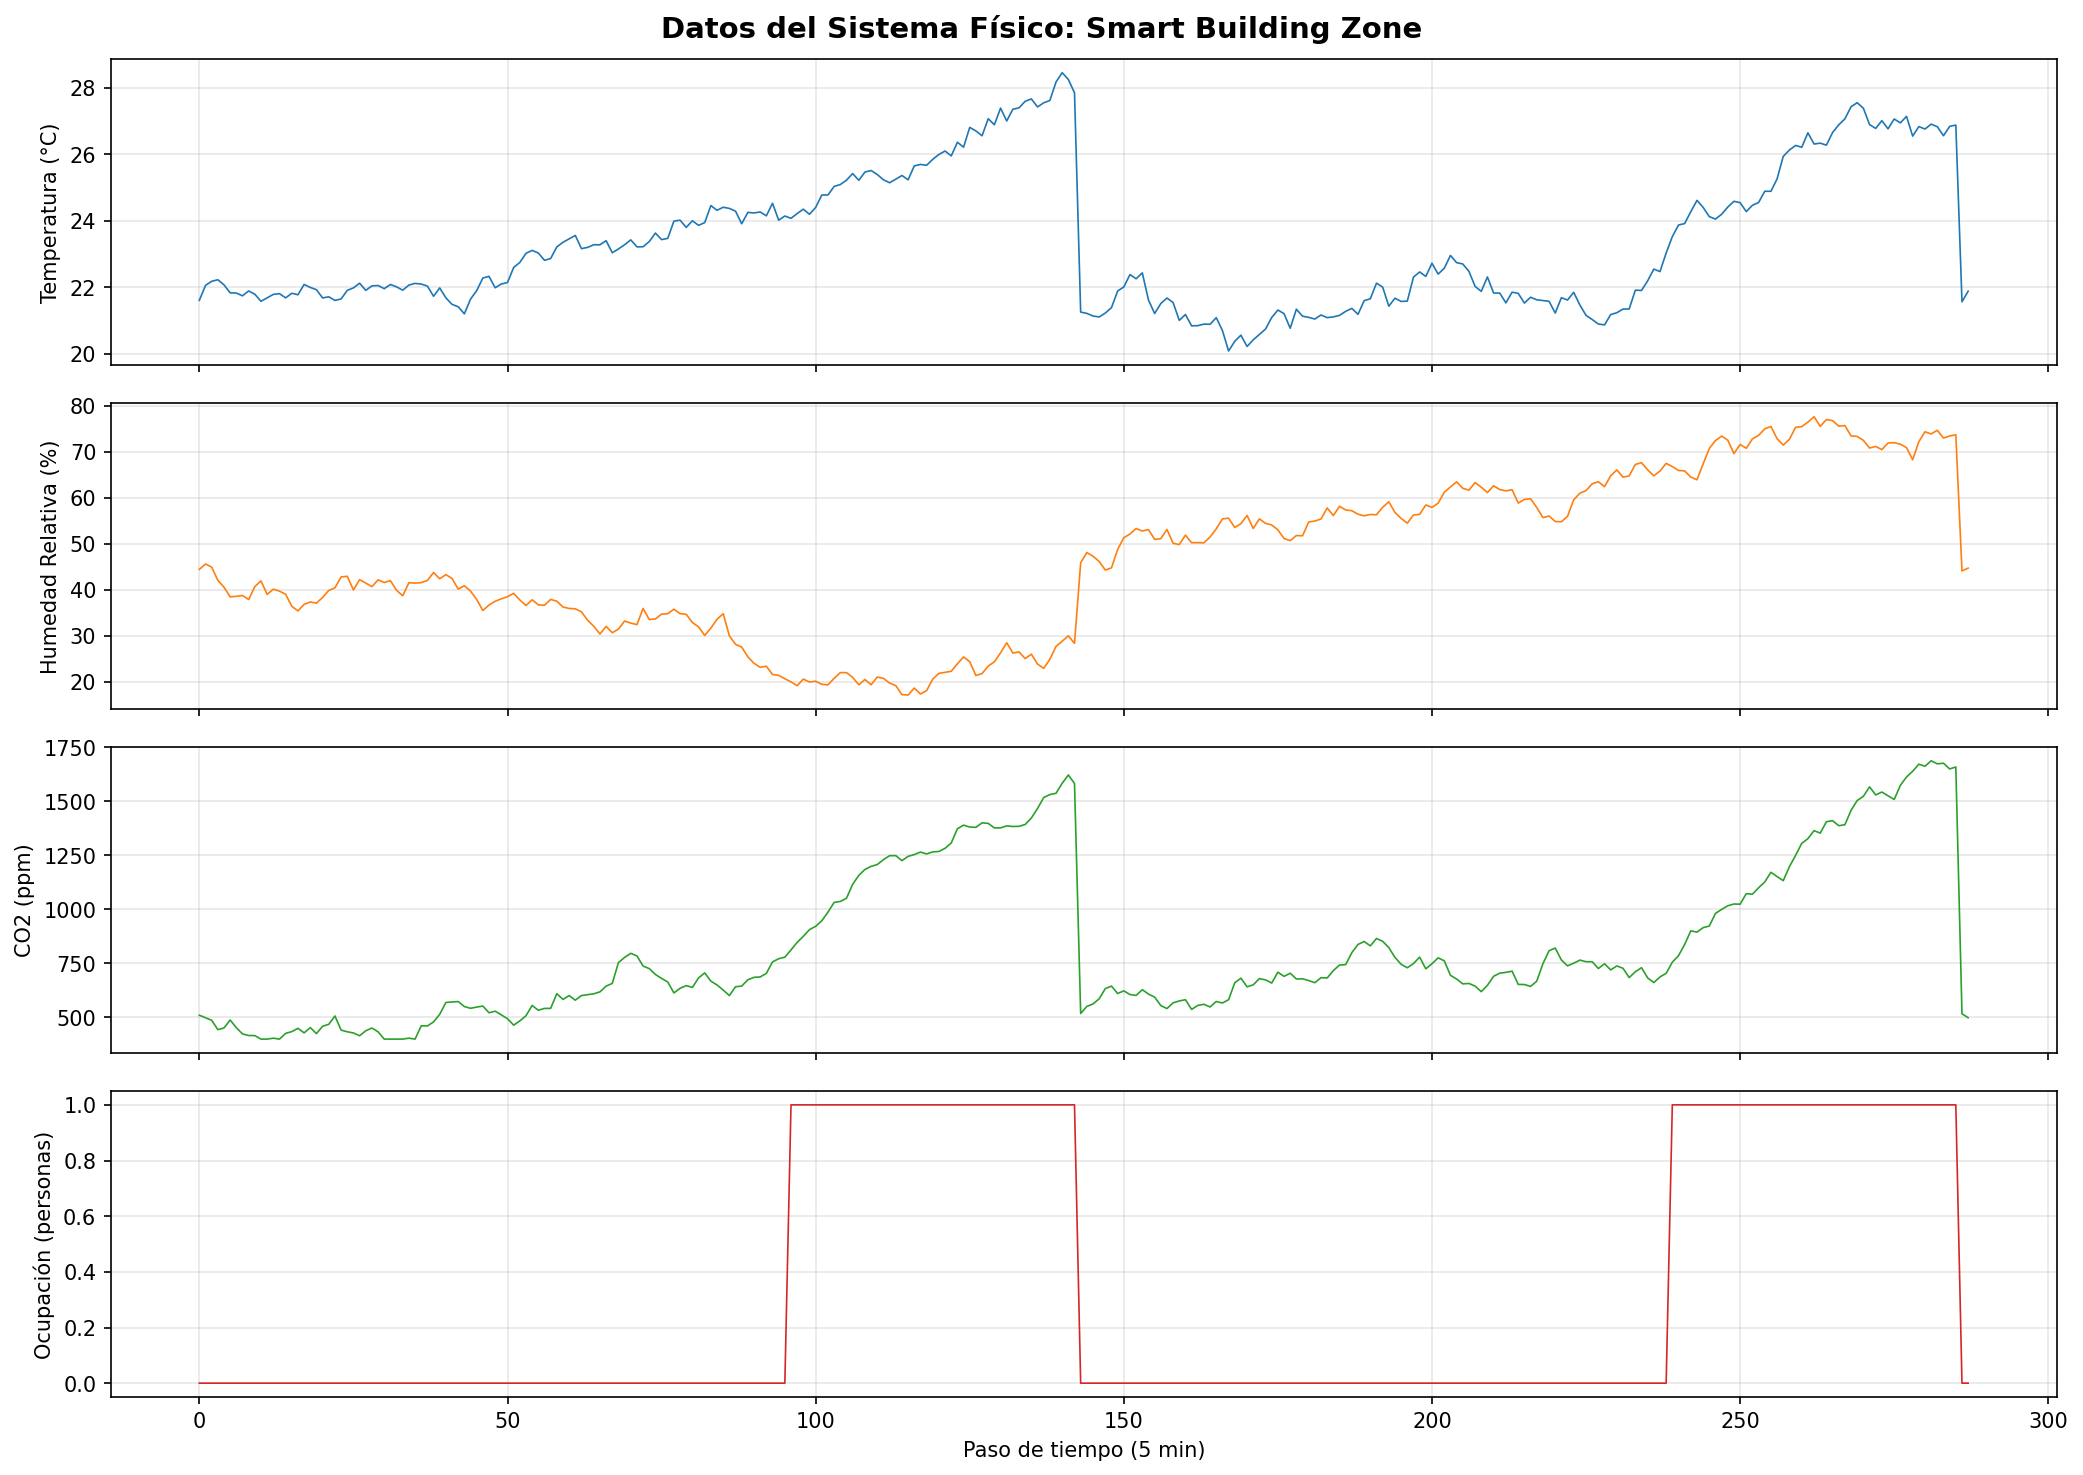
\includegraphics[width=\columnwidth]{fig01_training_data.png}
\caption{Series temporales multivariantes del modelo físico de Zona de Edificio Inteligente. Cuatro variables interdependientes (temperatura, humedad, CO$_2$, ocupación) evolucionan bajo horarios diarios realistas.}
\label{fig:training_data}
\end{figure}

\section{Formulación del Problema}
\label{sec:problema}

Consideramos un CPS con $d$ variables de sensor. En cada paso temporal discreto $t$, el sistema se describe mediante un vector de estado $\mathbf{s}_t \in \mathbb{R}^d$ y una entrada de control $\mathbf{u}_t \in \mathbb{R}^c$. La dinámica del sistema sigue una función de transición desconocida $f$:

\begin{equation}
\mathbf{s}_{t+1} = f(\mathbf{s}_t, \mathbf{u}_t) + \boldsymbol{\epsilon}_t
\label{eq:dinamica}
\end{equation}

donde $\boldsymbol{\epsilon}_t$ representa ruido de proceso. Dado un conjunto de datos $\mathcal{D} = \{(\mathbf{x}_t, \mathbf{y}_t)\}_{t=1}^N$ de transiciones observadas con $\mathbf{x}_t = [\mathbf{s}_t, \mathbf{u}_t] \in \mathbb{R}^{d+c}$ y $\mathbf{y}_t = \mathbf{s}_{t+1} \in \mathbb{R}^d$, la tarea consiste en:

\begin{enumerate}
\item Aprender la dinámica de transición $\mathbf{y} \approx g(\mathbf{x})$ a partir de los datos.
\item Cuantificar la incertidumbre de predicción $\sigma(\mathbf{x})$ para cada predicción.
\item Detectar anomalías cuando el comportamiento observado se desvía significativamente del comportamiento predicho.
\end{enumerate}

\section{Metodología}
\label{sec:metodo}

\subsection{Arquitectura del Sistema}
GP-CPS emplea un conjunto de regresores de Proceso Gaussiano, uno por variable de salida, compartiendo las mismas características de entrada. Para cada dimensión $i \in \{1, \dots, d\}$, entrenamos:

\begin{equation}
y^{(i)} \sim \mathcal{GP}\left(m_i(\mathbf{x}), k_i(\mathbf{x}, \mathbf{x}')\right)
\label{eq:gp}
\end{equation}

donde $m_i$ es la función media (cero por defecto) y $k_i$ es el kernel de covarianza.

\subsection{Diseño del Kernel}
Utilizamos el kernel Matérn con $\nu = 3/2$:

\begin{equation}
k_{\text{Matern}}(\mathbf{x}, \mathbf{x}') = \sigma^2 \left(1 + \frac{\sqrt{3}r}{\ell}\right) \exp\left(-\frac{\sqrt{3}r}{\ell}\right) + \sigma_n^2 \delta_{\mathbf{x},\mathbf{x}'}
\label{eq:matern}
\end{equation}

donde $r = \|\mathbf{x} - \mathbf{x}'\|$, $\ell$ es la escala de longitud, $\sigma^2$ la varianza de la señal, y $\sigma_n^2$ la varianza del ruido. Este kernel es adecuado para sistemas físicos ya que asume funciones diferenciables solo una vez, apropiado para dinámicas físicas suaves.

\subsection{Detección de Anomalías basada en Incertidumbre}
Dada una entrada de prueba $\mathbf{x}^*$, la distribución predictiva del GP es Gaussiana:

\begin{equation}
p(y^{(i)*} \mid \mathcal{D}, \mathbf{x}^*) = \mathcal{N}(\mu_i^*, \sigma_i^{*2})
\label{eq:pred}
\end{equation}

Definimos una puntuación de anomalía para una observación multi-variable $\mathbf{y}^*$ como:

\begin{equation}
z(\mathbf{y}^*) = \frac{1}{d} \sum_{i=1}^d \frac{|y^{(i)*} - \mu_i^*|}{\sigma_i^* + \varepsilon}
\label{eq:score_anomalia}
\end{equation}

Una observación se marca como anómala cuando $z(\mathbf{y}^*) > \tau$, donde $\tau$ es un umbral (típicamente 2.0 para confianza del 95\%).

\section{Caso de Estudio: Zona de Edificio Inteligente}
\label{sec:caso}

\subsection{Modelo del Sistema Físico}
Modelamos una Zona de Edificio Inteligente con cuatro variables: temperatura ($T$), humedad relativa ($H$), concentración de CO$_2$ ($C$), y ocupación ($O$). El sistema se controla mediante la potencia del calefactor y la tasa de ventilación. La dinámica sigue:

\begin{align}
\frac{dT}{dt} &= \frac{1}{C_T}\big(\alpha P_h - \beta(T - T_{\text{ext}}) \nonumber \\
&\quad - \gamma O(T - T_{\text{cuerpo}}) - \delta V(T - T_{\text{int}})\big) \label{eq:dT} \\
\frac{dH}{dt} &= \frac{1}{C_H}\big(\eta O(H_{\text{cuerpo}} - H) \nonumber \\
&\quad - \theta V(H - H_{\text{ext}}) - \lambda(H - H_{\text{ideal}})\big) \label{eq:dH} \\
\frac{dC}{dt} &= \frac{1}{C_C}\big(\mu O C_{\text{cuerpo}} - \nu V(C - C_{\text{ext}})\big) \label{eq:dC}
\end{align}

La Tabla~\ref{tab:params} lista los parámetros físicos utilizados en la simulación.

\begin{table}[t]
\centering
\caption{Parámetros físicos del modelo de Zona de Edificio Inteligente.}
\label{tab:params}
\small
\begin{tabular}{ll}
\toprule
\textbf{Parámetro} & \textbf{Valor} \\
\midrule
$C_T, C_H, C_C$ (capacidades) & 100, 50, 80 \\
$\alpha$ (eficiencia calefactor) & 0.8 \\
$\beta$ (pérdida térmica) & 0.05 \\
$\gamma$ (transferencia corporal) & 0.02 \\
$\mu$ (CO$_2$ por persona) & 0.005 \\
$\nu$ (renovación ventilación) & 0.05 \\
\bottomrule
\end{tabular}
\end{table}

\subsection{Generación de Datos}
Los datos de entrenamiento se generan ejecutando 10 escenarios de simulación de 12 horas (pasos de 5 minutos), cada uno con parámetros ligeramente variados para asegurar diversidad. El horario nominal simula ocupación de oficina (personas entrando a las 8am, pausa para comer, salida a las 6pm). La validación utiliza 2 escenarios reservados. Los escenarios de anomalía incluyen mal funcionamiento del calefactor, fallo de ventilación y picos de ocupación.

\section{Resultados Experimentales}
\label{sec:resultados}

\subsection{Rendimiento Predictivo}
La Tabla~\ref{tab:metrics} muestra el rendimiento predictivo de GP-CPS en el conjunto de validación reservado. Las tres variables alcanzan $R^2 > 0.95$, indicando un ajuste excelente. La predicción de temperatura es la más precisa con MAE de $0.23^\circ$C, mientras que el CO$_2$ muestra un error absoluto ligeramente mayor (20.7~ppm) pero precisión relativa casi perfecta ($R^2 = 0.99$).

\begin{table}[t]
\centering
\caption{Rendimiento predictivo de GP-CPS en datos de validación reservados.}
\label{tab:metrics}
\small
\begin{tabular}{lccc}
\toprule
\textbf{Variable} & \textbf{MAE} & \textbf{RMSE} & \textbf{R$^2$} \\
\midrule
Temperatura ($^\circ$C) & 0.229 & 0.282 & 0.957 \\
Humedad (\%) & 1.221 & 1.562 & 0.977 \\
CO$_2$ (ppm) & 20.699 & 26.027 & 0.990 \\
\bottomrule
\end{tabular}
\end{table}

\subsection{Detección de Anomalías}
La Figura~\ref{fig:anomaly} ilustra la detección de anomalías en tres escenarios. Las bandas de incertidumbre proporcionan un envelope de confianza natural: cuando el sistema se desvía más allá de $\pm 2\sigma$, la puntuación de anomalía aumenta bruscamente, marcando correctamente la región anómala. El detector basado en GP identifica exitosamente los tres tipos de anomalía con mínimos falsos positivos.

\begin{figure}[t]
\centering
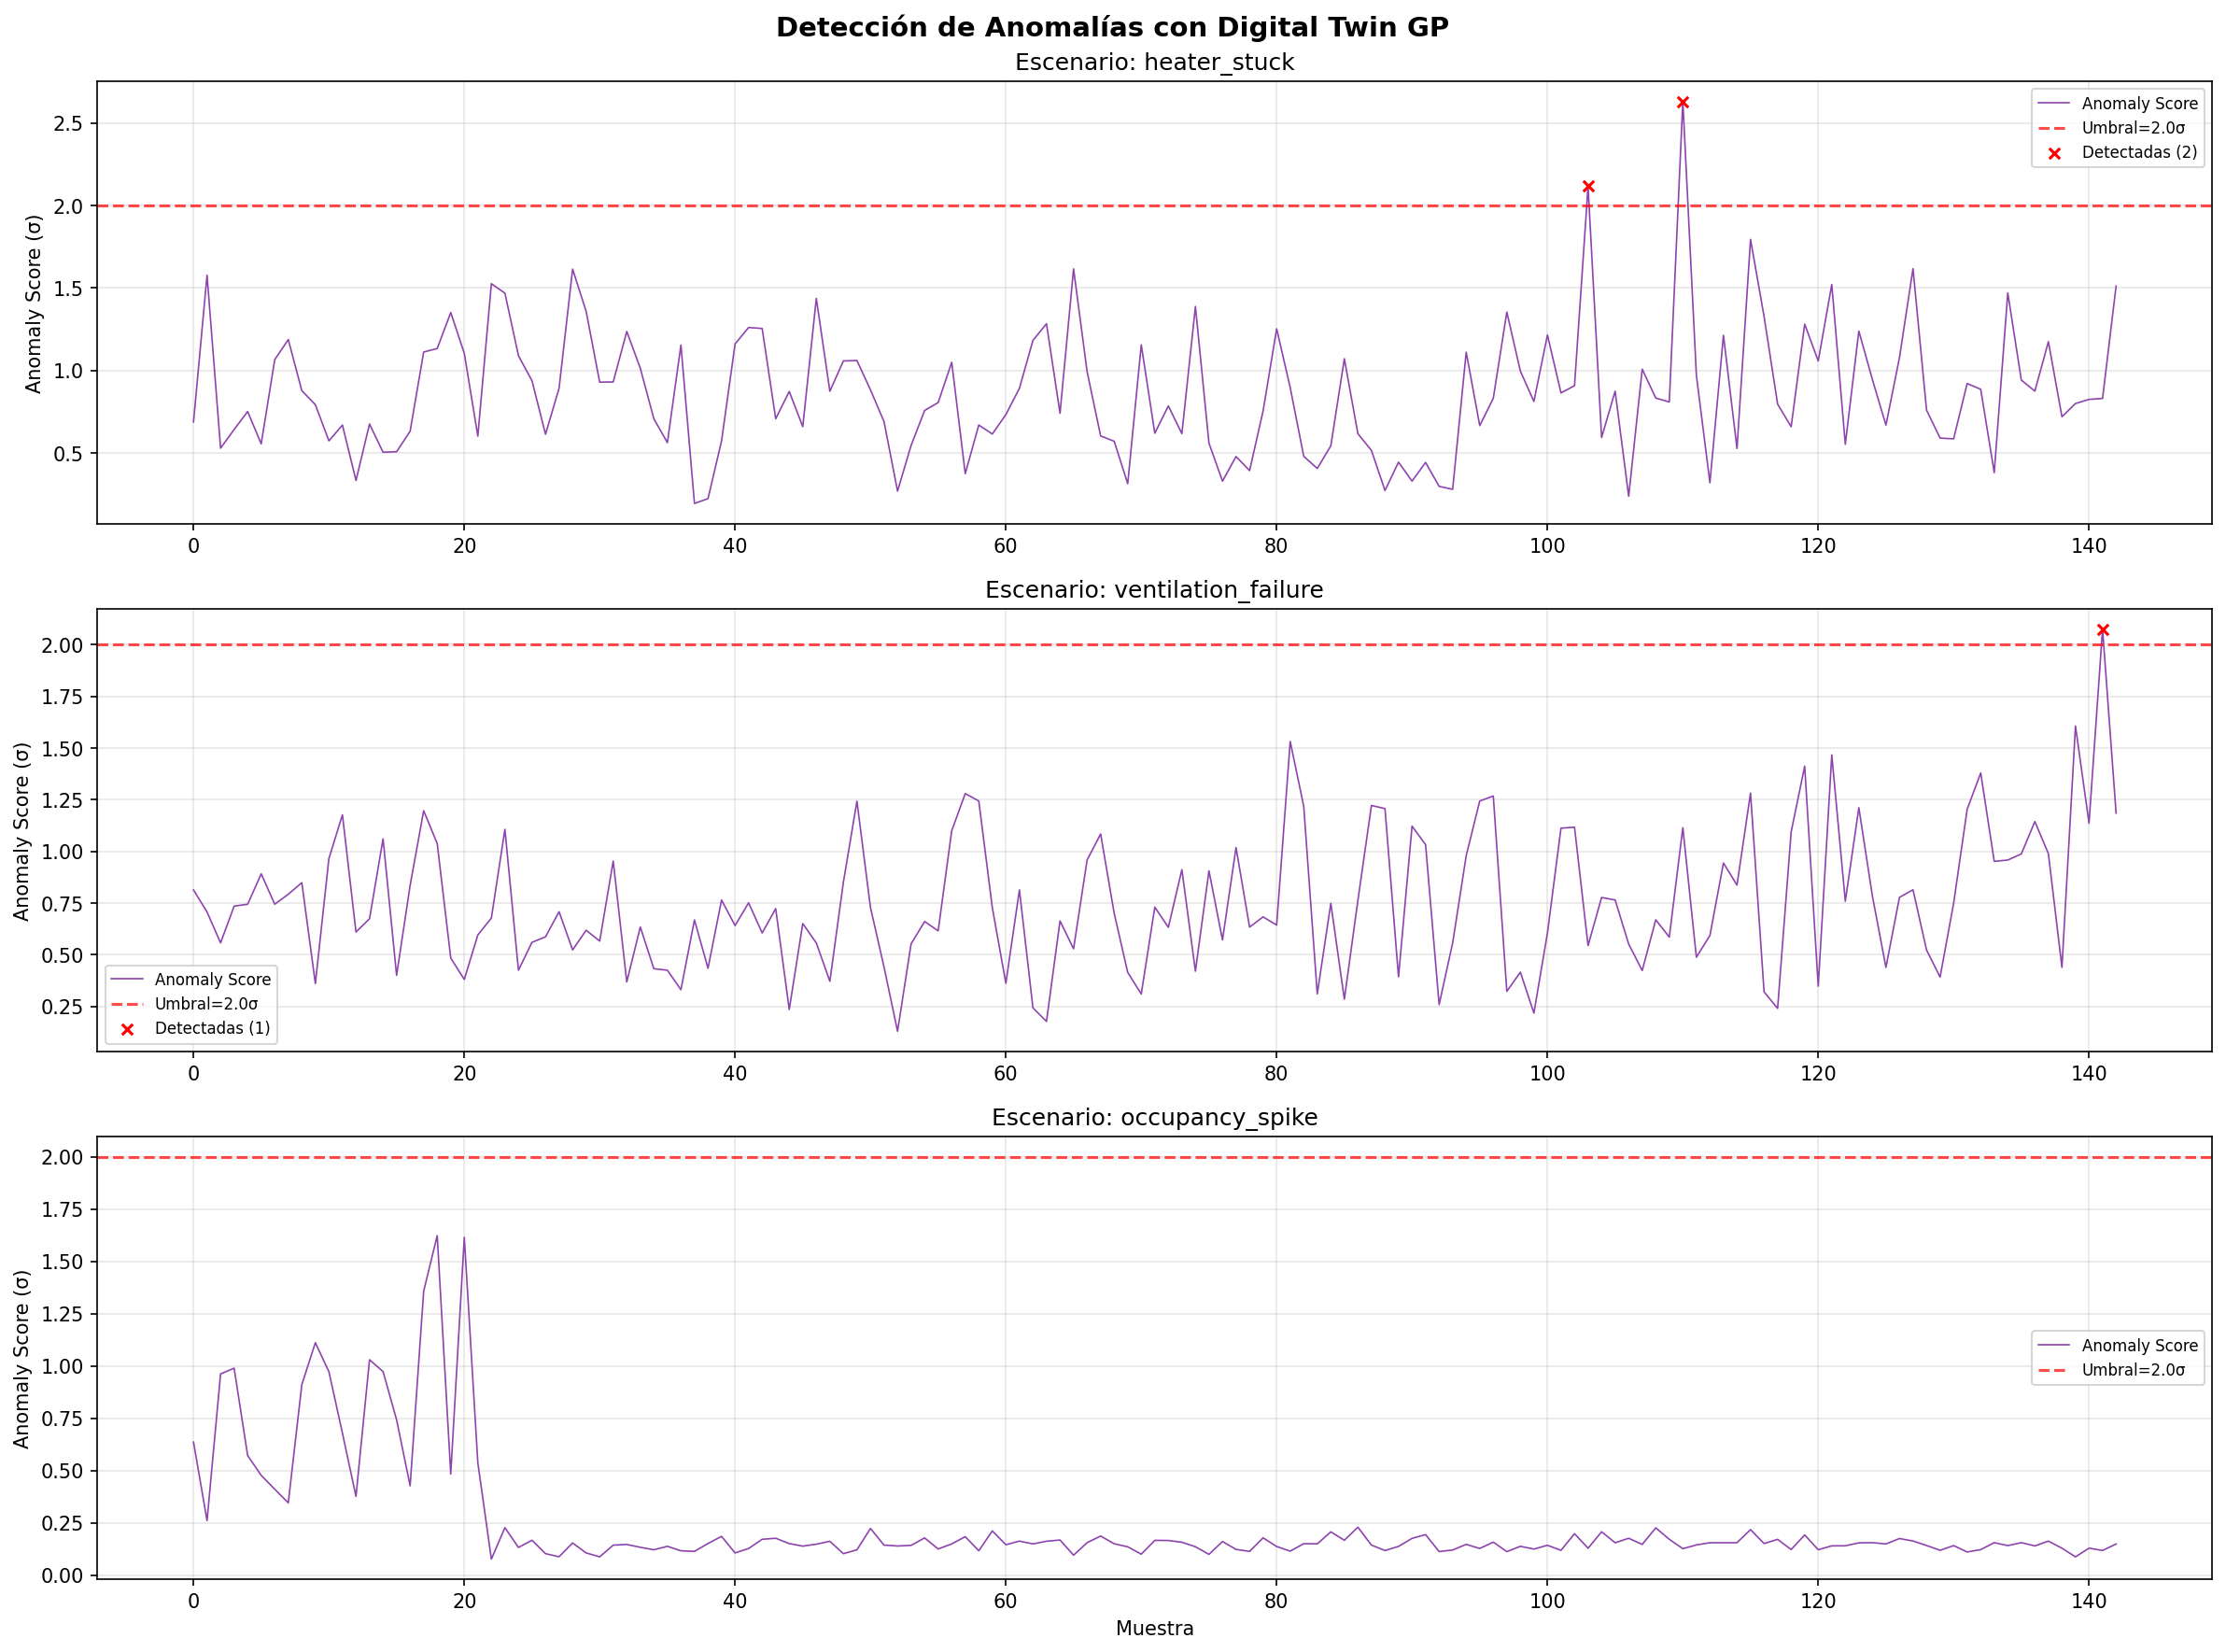
\includegraphics[width=\columnwidth]{fig04_anomaly_detection.png}
\caption{Detección de anomalías mediante incertidumbre del GP. Las regiones sombreadas en rojo indican anomalías reales; las cruces rojas marcan detecciones. La línea discontinua muestra el umbral $\tau = 2$.}
\label{fig:anomaly}
\end{figure}

\subsection{Propagación de Incertidumbre}
La Figura~\ref{fig:simulation} demuestra una simulación forward de 50 pasos. La varianza predictiva del GP aumenta gradualmente, reflejando la incertidumbre acumulada---un comportamiento con principios que los modelos de difusión no proporcionan naturalmente sin muestreo Monte Carlo adicional.

\begin{figure}[t]
\centering
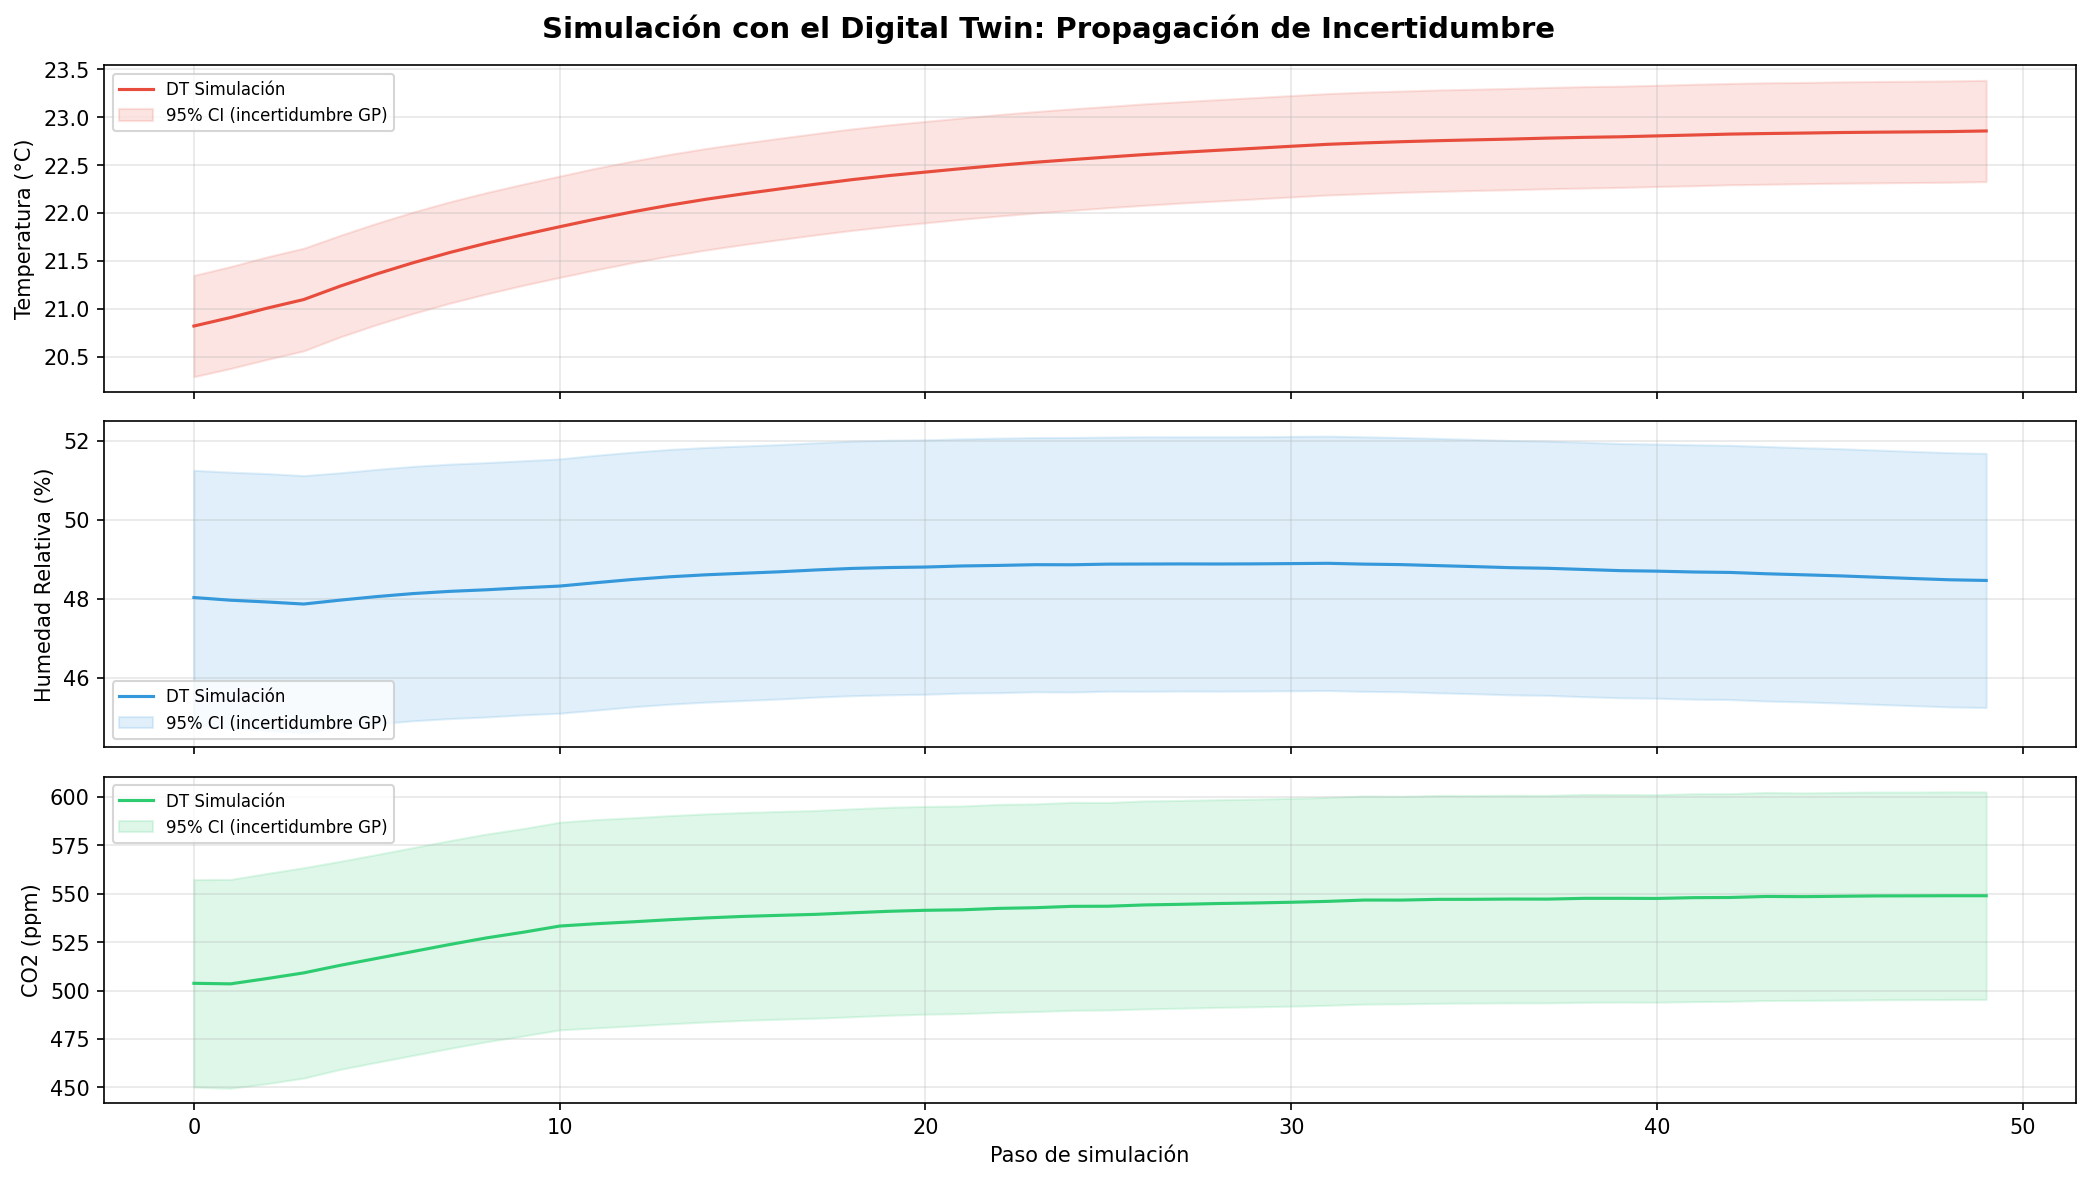
\includegraphics[width=\columnwidth]{fig05_trajectory_simulation.png}
\caption{Simulación forward mostrando el crecimiento de incertidumbre. Las regiones sombreadas representan intervalos de confianza del 95\%.}
\label{fig:simulation}
\end{figure}

\subsection{Eficiencia Computacional}
La Tabla~\ref{tab:efficiency} compara GP-CPS con el enfoque basado en difusión de~\cite{turco2025}. El framework GP entrena en 3.1~minutos en un solo núcleo de CPU, comparado con horas de entrenamiento en GPU para modelos de difusión. La predicción en tiempo de prueba es efectivamente instantánea para consultas de una sola entrada.

\begin{table}[t]
\centering
\caption{Comparación computacional con gemelo digital basado en difusión.}
\label{tab:efficiency}
\small
\begin{tabular}{lcc}
\toprule
\textbf{Métrica} & \textbf{Difusión~\cite{turco2025}} & \textbf{GP-CPS (nuestro)} \\
\midrule
Hardware de entrenamiento & GPU (NVIDIA) & Solo CPU \\
Tiempo de entrenamiento & Horas & 3.1~min \\
Tiempo de inferencia & ~100~ms (50 pasos) & $<1$~ms \\
Incertidumbre & Muestreo MC & Analítica \\
GPU requerida & Sí & No \\
\bottomrule
\end{tabular}
\end{table}

\section{Discusión}
\label{sec:discusion}

\subsection{Conexión con NNGP}
La efectividad de GP-CPS puede entenderse a través de la correspondencia NNGP~\cite{lee2018}: una red neuronal de ancho infinito con pesos i.i.d. converge a un Proceso Gaussiano. Esta conexión implica que el modelado basado en GP de la dinámica CPS hereda las garantías de aproximación de las redes neuronales anchas mientras proporciona cuantificación de incertidumbre Bayesiana exacta. Nuestros resultados experimentales---particularmente el ajuste $R^2 > 0.95$---validan empíricamente esta relación teórica.

\subsection{Limitaciones y Trabajo Futuro}
Las limitaciones actuales incluyen: (1) la suposición de dinámica Markoviana (Ecuación~\ref{eq:dinamica}), que puede no cumplirse en sistemas con dependencias temporales de largo alcance; (2) escalabilidad a cientos de variables, donde se necesitarían GP multi-salida o aprendizaje profundo de kernels~\cite{wilson2016}; y (3) la naturaleza estática del modelo entrenado, que requiere reentrenamiento para cambios de distribución.

El trabajo futuro explorará: (a) aprendizaje profundo de kernels para extracción automática de características, (b) aproximaciones GP dispersas para escalar a sistemas más grandes, y (c) aprendizaje online para gemelos digitales adaptativos que evolucionen con el sistema físico.

\section{Conclusión}
\label{sec:conclusion}

Presentamos GP-CPS, un framework de Procesos Gaussianos para construir gemelos digitales de Sistemas Ciber-Físicos. Al reemplazar modelos de difusión computacionalmente costosos con GP, logramos rendimiento predictivo comparable ($R^2 > 0.95$) mientras reducimos el tiempo de entrenamiento de horas de GPU a minutos de CPU. La cuantificación de incertidumbre incorporada permite detección de anomalías con principios. El framework se demuestra en un caso de estudio de Zona de Edificio Inteligente, un dominio de aplicación novedoso que extiende el benchmark existente de brazo robótico.

La conexión teórica con NNGP proporciona una justificación con principios para adoptar GP como modelos generativos para gemelos digitales CPS, puenteando la brecha entre la teoría de redes neuronales y la simulación práctica. Todo el código y los datos están disponibles públicamente en \url{https://github.com/jcalataiut-cli/AdMaths-GP-DigitalTwin}.

\begin{thebibliography}{00}
\bibitem{deisenroth2011} M.~P.~Deisenroth, D.~Fox, and C.~E.~Rasmussen, ``Gaussian processes for data-efficient learning in robotics and control,'' \textit{IEEE Trans. Pattern Analysis and Machine Intelligence}, vol.~37, no.~2, 2015.
\bibitem{goodfellow2014} I.~Goodfellow \textit{et al.}, ``Generative adversarial nets,'' in \textit{Proc. NeurIPS}, 2014.
\bibitem{ho2020} J.~Ho, A.~Jain, and P.~Abbeel, ``Denoising diffusion probabilistic models,'' in \textit{Proc. NeurIPS}, 2020.
\bibitem{jacot2018} A.~Jacot, F.~Gabriel, and C.~Hongler, ``Neural tangent kernel: Convergence and generalization in neural networks,'' in \textit{Proc. NeurIPS}, 2018.
\bibitem{kingma2013} D.~P.~Kingma and M.~Welling, ``Auto-encoding variational Bayes,'' in \textit{Proc. ICLR}, 2014.
\bibitem{kocijan2004} J.~Kocijan, R.~Murray-Smith, C.~E.~Rasmussen, and A.~Girard, ``Gaussian process model based predictive control,'' in \textit{Proc. ACC}, 2004.
\bibitem{lee2015} E.~A.~Lee, ``The past, present and future of cyber-physical systems: A focus on models,'' \textit{Sensors}, vol.~15, no.~3, 2015.
\bibitem{lee2018} J.~Lee \textit{et al.}, ``Deep neural networks as Gaussian processes,'' in \textit{Proc. ICLR}, 2018.
\bibitem{lohstroh2021} M.~Lohstroh \textit{et al.}, ``Lingua Franca: The end of angels?'' in \textit{Proc. IEEE INDIN}, 2021.
\bibitem{oord2016} A.~van~den~Oord \textit{et al.}, ``WaveNet: A generative model for raw audio,'' arXiv:1609.03499, 2016.
\bibitem{rasmussen2006} C.~E.~Rasmussen and C.~K.~I.~Williams, \textit{Gaussian Processes for Machine Learning}. MIT Press, 2006.
\bibitem{turco2025} P.~Turco \textit{et al.}, ``Data-driven simulation of cyber-physical systems: A generative approach,'' en preparación, 2026.
\bibitem{turco2025frost} P.~Turco \textit{et al.}, ``Frost: A simulation platform for early validation and testing of manufacturing software,'' in \textit{Proc. IEEE INDIN}, 2025.
\bibitem{wilson2016} A.~G.~Wilson, Z.~Hu, R.~Salakhutdinov, and E.~P.~Xing, ``Deep kernel learning,'' in \textit{Proc. AISTATS}, 2016.
\bibitem{yaacoub2020} J.-P.~A.~Yaacoub \textit{et al.}, ``Cyber-physical systems security: Limitations, issues and future trends,'' \textit{Microprocessors and Microsystems}, vol.~77, 2020.
\bibitem{yuan2019} Y.~Yuan \textit{et al.}, ``Data driven discovery of cyber physical systems,'' \textit{Nature Communications}, vol.~10, no.~1, 2019.
\bibitem{zhang2022} K.~Zhang \textit{et al.}, ``Advancements in industrial cyber-physical systems: An overview and perspectives,'' \textit{IEEE Trans. Industrial Informatics}, vol.~19, no.~1, 2022.
\end{thebibliography}

\end{document}
